\section{\Po s}
\label{s:numerics}

The simple structure of the symmetry-reduced dynamics allows us to
determine the \rpo s of the \twomode\ system by means of a Poincar\'e
section and a return map. We illustrate this procedure in
\reffig{fig:psectandretmap}. Starting with an initial point close to the
\REQV{}{}, we compute a long, symmetry-reduced ergodic trajectory by integrating
\refeq{e-so2red1stmode} and record where it crosses the Poincar\'e section, which we
define as the plane that contains \REQV{}{} and is spanned the imaginary part of its unstable stability
eigenvector and $\hat{y}_2$.
\BB{2014-11-06}{It includes $\hat{y}_2$ direction, a bit random but it doesn't
matter that much because attractor is super thin, I think the figure does the
job (everything is there, it's not a projection etc.), but you can add if you
think it's necessary.}\DB{2014-11-10}{Dropped color coding from main text since it's already in the figure.
Reworded a little to make Poincare section definition more precise and make our work repeatable. Also see comments in figure caption.}
We then project these points onto a basis $(v_1, v_2)$, which
spans the Poincar\'e section and fit cubic splines to the data as shown in \reffig{fig:psectandretmap}\,(b).
We then construct a return map along this curve and express this in terms of the distance $s$ from \REQV{}{}
as measured by the arc length along the cubic spline fit. The resulting map, which is shown in
\reffig{fig:psectandretmap}\,(c), is unimodal with a sharp cusp located at its critical point.
Note that the region $s \in (0, 0.6)$ corresponds to
the neighborhood of the \reqv\  and is only visited transiently. Once the dynamics fall onto the chaotic
attractor, this region is never visited again. Removing this region from the return map, we
obtain the return map shown in \reffig{fig:psectandretmap}\,(d), which we can then use to determine the
accessible \rpo s  with their respective binary symbol sequences.

\begin{figure}
\centering
  (a) 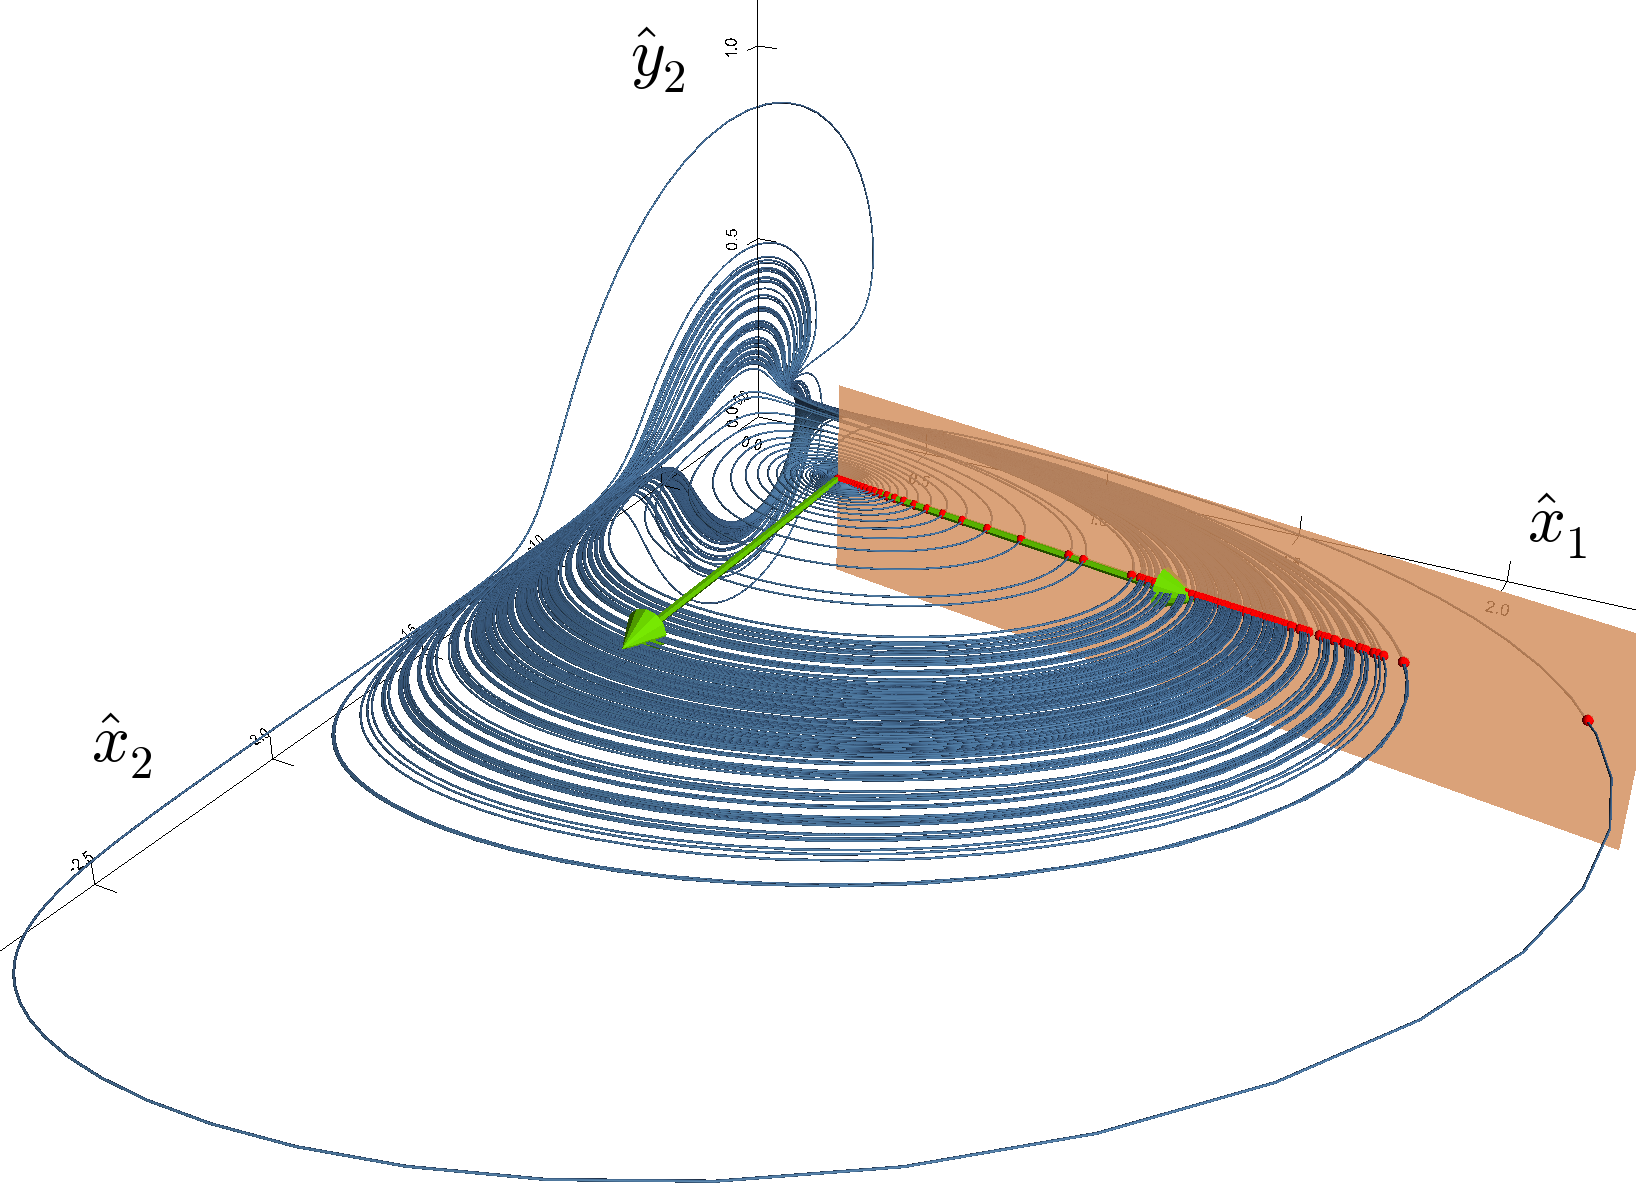
\includegraphics[width=0.45\textwidth]{BBpsecthd} \\
  (b) 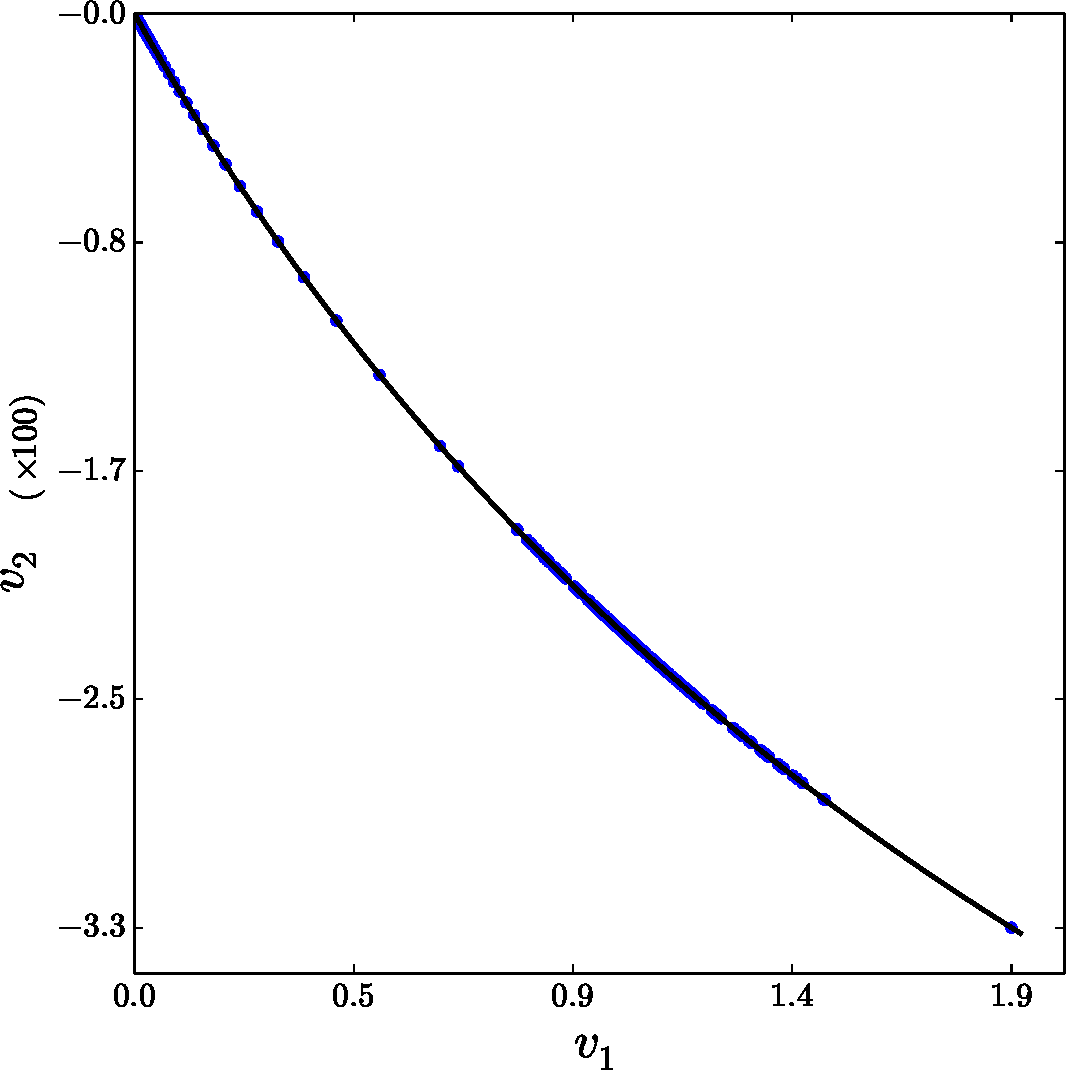
\includegraphics[height=0.19\textwidth]{BBpsectonslice}
  (c) 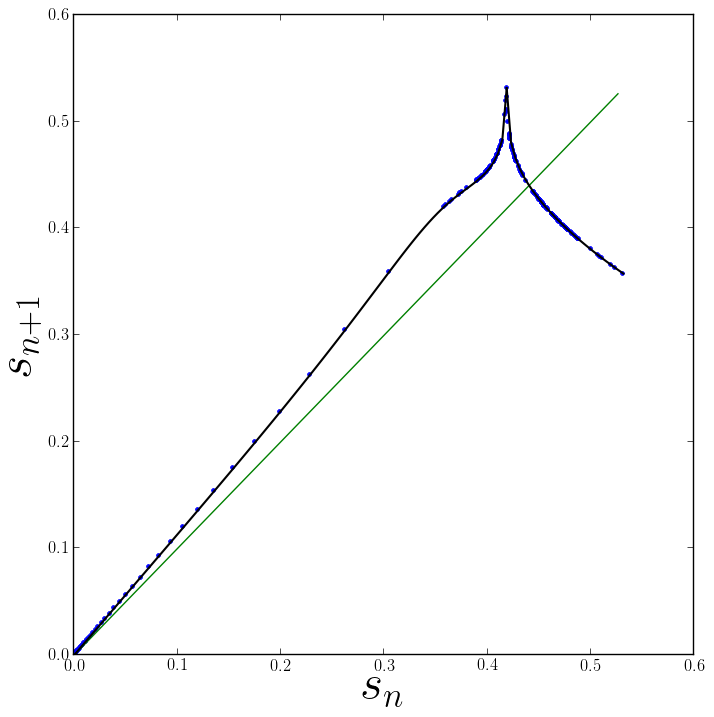
\includegraphics[height=0.19\textwidth]{BBretmaponslice} \\
  (d) 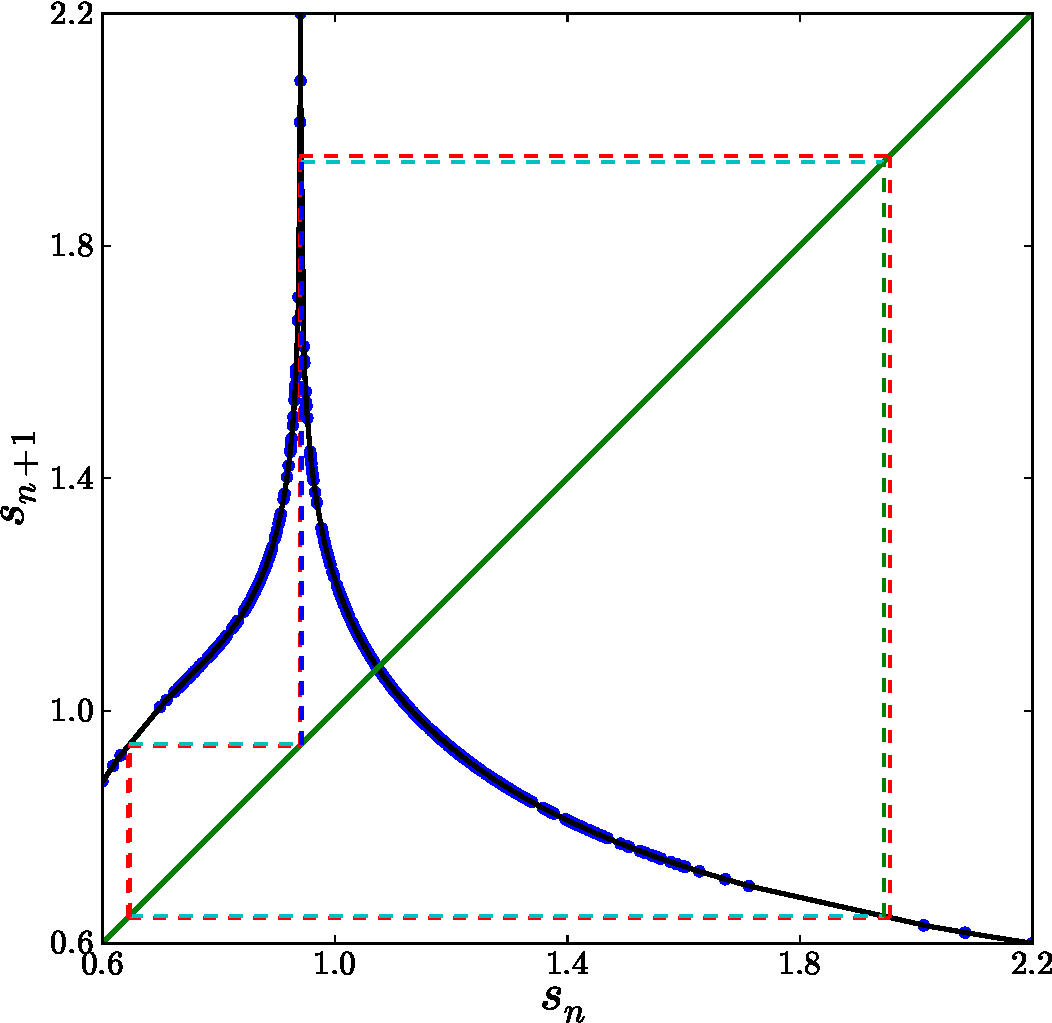
\includegraphics[width=0.45\textwidth]{BBretmaponsliceZoom}
\caption{(Color online)
         (a) Symmetry-reduced ergodic trajectory within the slice hyperplane (blue).
			Green arrows indicate the real and imaginary parts of the complex eigenvectors
			$v_u$ that span the unstable manifold of \REQV{}{}. The Poincar\'e section, which contains \REQV{}{} and is spanned by
			$\Im[v_u]$ and $\hat{y}_2$, is visualized as a transparent plane. Points where the flow crosses
			the are marked in red.
		 (b) The Poincar\'e section which includes the \REQV{}{} and $v_u$ projected
			on to the basis within the plane shown in (a)\DB{2014-11-3}{description of what $v_1$ and $v_2$
			are is not clear here... I mean, I think I know what you are trying to say, but it's not explicit.
			Also, might be useful to plot \REQV{}{} in a different color here.}. Included is a
            transient trajectory initiated close to \REQV{}{}. Note that
		  	the vertical axis is magnified by $100$.
		 (c) The Poincar\'e return map for the Poincar\'e section (b). The distances between points
		are given in term of the arc length $s$ along the curve in (b).\DB{}{Double check this statement for correctness.}
		 (d) The return map without the transient points framed by
            orbit of the critical point.
		 	Dashed lines show the 3-cycles \cycle{001} (red) and \cycle{011} (cyan).}
%\ES{on my screen, cyan line appears to change color in vertical parts of the figure.}
%I commented out this edit because it was preventing the file from compiling.
\label{fig:psectandretmap}
\end{figure}

The unimodal return map of \reffig{fig:psectandretmap} diverges around
$s \approx 0.98$ and this neighborhood is visited very rarely by the flow. We
took the furthest point that is visited by the ergodic flow, $s_C=0.98102264$
as the critical point of this map and coded points to the left and right hand sides of this
point as `0' and `1', respectively, to construct binary symbolic dynamics.
Accessible periodic orbits are then those with the topological coordinates
less than that of this critical point. We skip the technical details
regarding symbolic dynamics and kneading theory in this tutorial since
there is a rich literature on these topics and we do not employ any novel
symbolic dynamics technique here. For a pedagogical introduction to the
subject, we refer the reader to \refrefs{devnmap, DasBuch}.

We are now going to summarize the procedure of locating \rpo s in the \statesp :
Suppose the binary itinerary
$\cycle{I_0 I_1 \dots\ I_{n-1}}, \mbox{where,}\, I_j = 0,1$
corresponds to an admissible `n-cycle', a \rpo\ that intersects our Poincar\'e
section n-times. We first find arc-lengths $\{s_0,\,s_1,\,\dots\,s_n\}$ that
constitutes this cycle on the return map \reffig{fig:psectandretmap}\,(d). We
then find corresponding reduced \statesp\ points
$\{\sspRed_0,\,\sspRed_1,\,\dots\, \sspRed_{n-1}\}$. Finally we integrate the
reduced flow and the phase \refeq{eq:so2reduced} starting from each found
reduced \statesp\ point $\sspRed_j$ until it returns to the Poincare\'e
section, and divide this trajectory into $N$ small pieces. As a result, we obtain
$n \times N$ \statesp\ points, durations and phase shifts
$\{\ssp_i^{(0)}\,,\,\zeit_i^{(0)}\,,\,\theta_i^{(0)}\}$ where
$i=1,\,2,\,\dots\,n \times N$ , which we feed into the multiple shooting Newton
solver (see \refappe{s:newton}) to precisely determine the \rpo , its period
and the associated phase shift. After finding $n \times N$ \statesp\ points
($\ssp_i$), flight times ($\zeit_i$), and phase shifts ($\theta_i$) associated
with the $n$ cycle, we then compute the flow Jacobian associated with each
piece $\jMps^{\zeit_i}(\ssp_i)$, using which we represent the Jacobian
associated with the \rpo\ as
\beq
    \jMpsRed=
    \matrixRep(\theta_{n \times N} ) \jMps^{\zeit_{n \times N}} (\ssp_{n \times N})
    \dots \,
    \matrixRep(\theta_2 ) \jMps^{\zeit_2} (\ssp_2)
    \matrixRep(\theta_1 ) \jMps^{\zeit_1} (\ssp_1) \, .
    \label{e-MultiShootJacobian}
\eeq
This construction \refeq{e-MultiShootJacobian} of Jacobian is equivalent to our
definition in \refeq{e-rpoJacobian}, since both group action $\LieEl$ and flow
Jacobian $\jMps$ are multiplicative and they commute with each other as a
consequence of $\LieEl$-equivariance of the flow. The form
\refeq{e-MultiShootJacobian} is essential in determining its eigenvalues
(Floquet multipliers) precisely for which we utilized periodic Schur
decomposition (\refappe{s:schur}) .


We found the admissible cycles of the
\twomode\ system upto the topological length 12. We listed binary itineraries
of of shortest $7$ \rpo s (with topological lengths up to 5), along with their
periods, phase shifts, Floquet multipliers, and Floquet exponents in
\reftab{t-rpofirst10}. In \reffig{f-2modesrpofirst4} we show shortest $4$ of
the \rpo s of the \twomode\ system within the first Fourier mode \slicePlane .
As seen from \reffig{f-2modesrpofirst4}, trajectories of \cycle{001} (red) and
\cycle{011} (cyan) almost overlap in a large region of the \statesp . This
behavior is also manifested in the return map of
\reffig{fig:psectandretmap}\,{d), where we have shown cycles \cycle{001} and
\cycle{011} with red and cyan respectively. This is a general property of the
\twomode\ cycles with odd topological lengths: They come in pairs with almost
equal leading (largest) Floquet exponents , see \reffig{f-2modes-lambdaDist}.
Floquet exponents ($\Lyap_j$) characterize the rate of expansion/contraction
of nearby perturbations to the \rpo s and are related to Floquet multipliers
($\ExpaEig_j$) by
\beq
    \Lyap_{\rpprime,j} = \frac{1}{\period{\rpprime}}
                         \ln | \ExpaEig_{\rpprime,j} |
                         \, , \quad j=1,2,\dots,d \, ,
\eeq
where the subscript $\rpprime$ indicates `prime \rpo\ $p$' and
$\period{\rpprime}$ is its period. Having computed periods, phase shifts,
and Floquet multipliers of \rpo s, we are now ready to calculate dynamical
averages and other statistical moments of observables using \cycForm s.

\begin{table}
	\caption{Itinerary, period ($T$), phase shift ($\theta$), 
			 Floquet multiplier ($\ExpaEig$), and Floquet exponent
			 ($\Lyap$) of the found \twomode\ \rpo s with topological
			 lengths up to $n = 5$, more (up to $n=12$) available 
			 upon request.}
	\begin{tabular}{c|c|c|c|c}
	Itinerary & $T$ & $\theta$ & $\ExpaEig$ & $\Lyap$ \\ 
	\hline
	1 & 3.64151221 & 0.08096967 & -1.48372354 &0.10834917 \\ 
	01 & 7.34594158 & -2.94647181 & -2.00054831 &0.09439516 \\ 
	001 & 11.07967801 & -5.64504385 & -55.77844510 &0.36295166 \\ 
	011 & 11.07958924 & -2.50675871 & 54.16250810 &0.36030117 \\ 
	0111 & 14.67951823 & -2.74691247 & -4.55966852 &0.10335829 \\ 
	01011 & 18.39155417 & -5.61529803 & -30.00633820 &0.18494406 \\ 
	01111 & 18.38741006 & -2.48213868 & 28.41893870 &0.18202976 \\ 
	\end{tabular}
	\label{t-rpofirst10}
\end{table}

\begin{figure}%[H]
\centering
 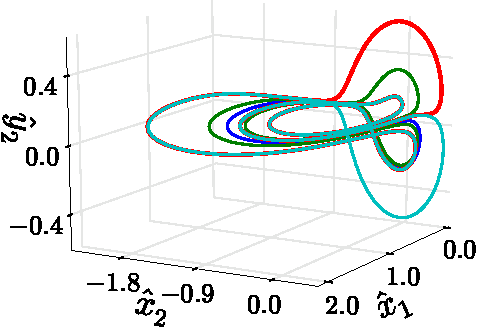
\includegraphics[width=0.45\textwidth]{2modesrpofirst4}
\caption{(Color online)
Shortest four \rpo s of the \twomode\ system: \cycle{1} (dark blue),
\cycle{01} (green), \cycle{001} (red), \cycle{011} (cyan). Note that \rpo
s \cycle{001} and \cycle{011} almost overlap everywhere except $\hat{x}_1
\approx 0$ .}
\label{f-2modesrpofirst4}
\end{figure}

\begin{figure}%[H]
\centering
 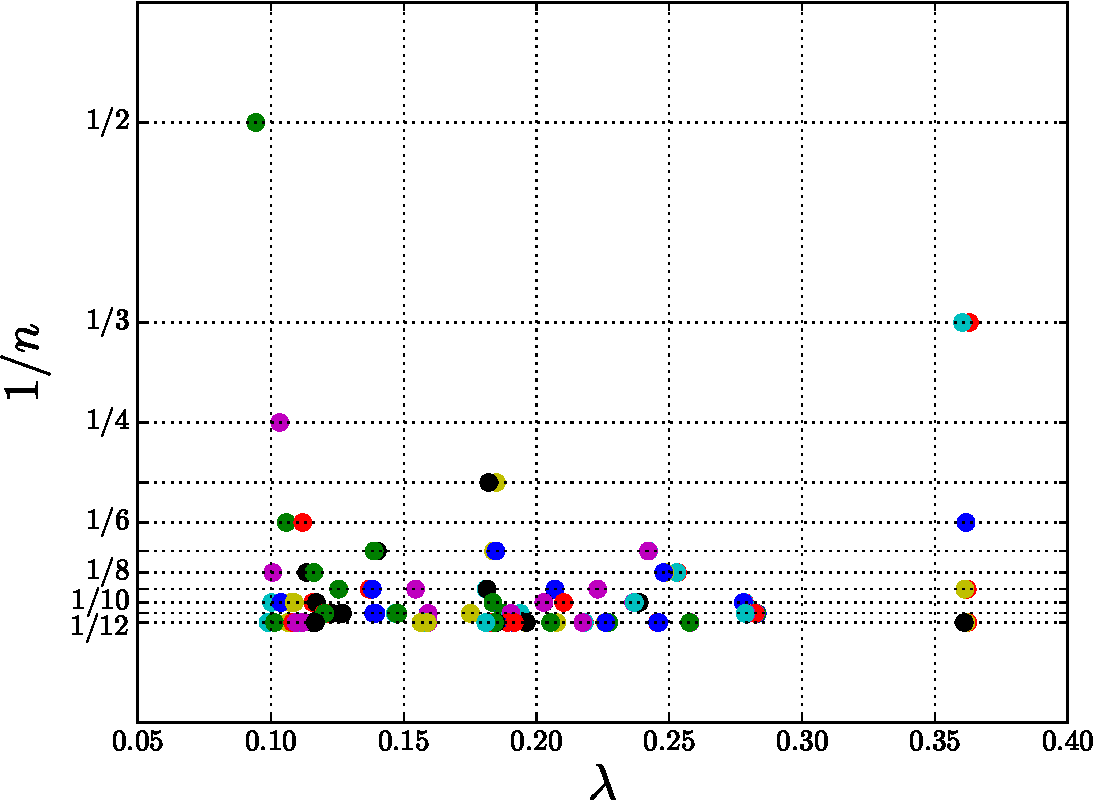
\includegraphics[width=0.45\textwidth]{2modes-lambdaDist}
\caption{(Color online)
        Distribution of the expanding Floquet exponents of all \twomode\ cycles with
         topological lengths $n$ from $2$ to $12$.}
\label{f-2modes-lambdaDist}
\end{figure}
